% Name: PRISMA flow diagram
% Description: How records were identified, screened, and included in a systematic review, with the count removed at each stage and why.
% Tags: PRISMA, systematic review, meta-analysis, flow diagram

\usetikzlibrary{arrows.meta, positioning, calc}

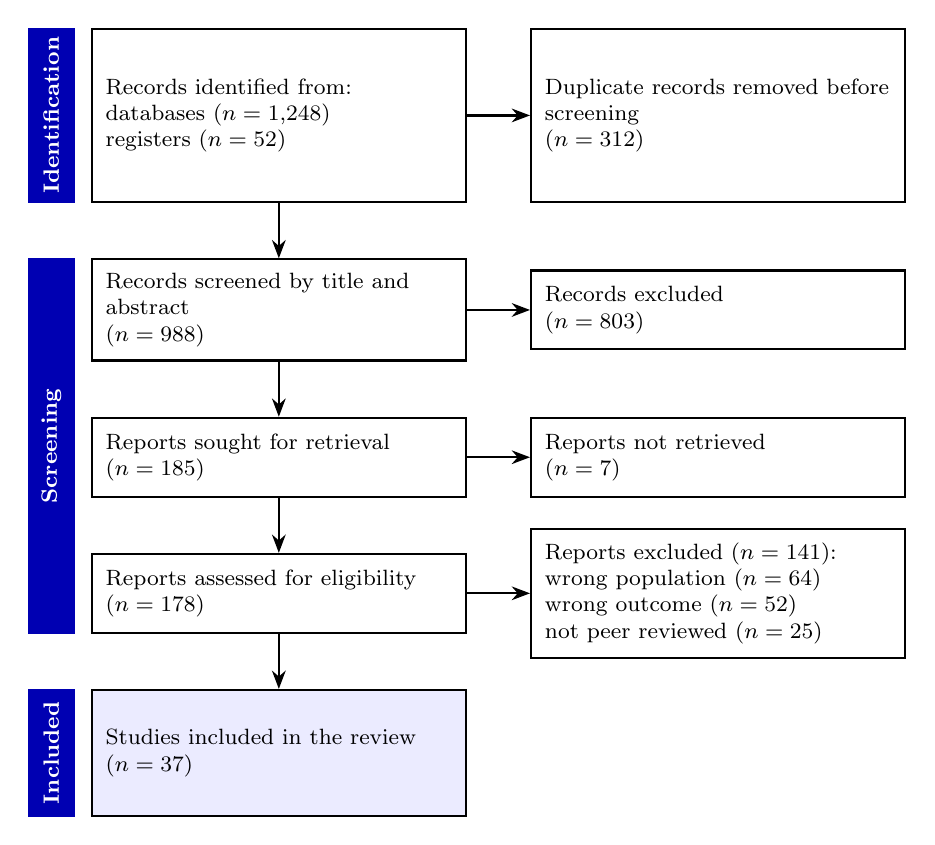
\begin{tikzpicture}[
  node distance=7mm and 8mm,
  every node/.style={font=\footnotesize},
  box/.style={draw, thick, text width=44mm, align=left, inner sep=5pt, minimum height=10mm},
  arrow/.style={-{Stealth}, thick},
]
  % Counts: 1,248 + 52 - 312 = 988; 988 - 803 = 185; 185 - 7 = 178; 178 - 141 = 37
  \node[box, minimum height=22mm] (found) {Records identified from:\\ databases ($n = 1{,}248$)\\ registers ($n = 52$)};
  \node[box, right=of found, minimum height=22mm] (dup) {Duplicate records removed before screening\\ ($n = 312$)};
  \node[box, below=of found] (screen) {Records screened by title and abstract\\ ($n = 988$)};
  \node[box, right=of screen] (ex1) {Records excluded\\ ($n = 803$)};
  \node[box, below=of screen] (sought) {Reports sought for retrieval\\ ($n = 185$)};
  \node[box, right=of sought] (miss) {Reports not retrieved\\ ($n = 7$)};
  \node[box, below=of sought] (full) {Reports assessed for eligibility\\ ($n = 178$)};
  \node[box, right=of full] (ex2) {Reports excluded ($n = 141$):\\ wrong population ($n = 64$)\\ wrong outcome ($n = 52$)\\ not peer reviewed ($n = 25$)};
  \node[box, below=of full, fill=blue!8, minimum height=16mm] (inc) {Studies included in the review\\ ($n = 37$)};

  \foreach \a/\b in {found/screen, screen/sought, sought/full, full/inc}
    \draw[arrow] (\a) -- (\b);
  \foreach \a/\b in {found/dup, screen/ex1, sought/miss, full/ex2}
    \draw[arrow] (\a) -- (\b);

  % Each phase bar runs from the top of its first box to the bottom of its last
  \foreach \top/\bot/\phase in {found/found/Identification, screen/full/Screening, inc/inc/Included} {
    \fill[blue!70!black] ([xshift=-8mm]\top.north west) rectangle ([xshift=-2mm]\bot.south west);
    \node[rotate=90, text=white, font=\footnotesize\bfseries] at ($([xshift=-5mm]\top.north west)!0.5!([xshift=-5mm]\bot.south west)$) {\phase};
  }
\end{tikzpicture}
